%% LyX 2.3.0 created this file.  For more info, see http://www.lyx.org/.
%% Do not edit unless you really know what you are doing.
\documentclass{article}
\usepackage{amsmath}
\usepackage{amsthm}
\usepackage{amssymb}
\usepackage{fontspec}
\setcounter{secnumdepth}{0}
\usepackage{mathtools}
\usepackage{cancel}
\usepackage{mathdots}
\usepackage{stmaryrd}
\usepackage{stackrel}
\usepackage{undertilde}
\usepackage{graphicx}
\PassOptionsToPackage{version=3}{mhchem}
\usepackage{mhchem}
\usepackage[unicode=true,
 bookmarks=false,
 breaklinks=true,pdfborder={0 0 0},pdfborderstyle={},backref=section,colorlinks=false]
 {hyperref}

\makeatletter
%%%%%%%%%%%%%%%%%%%%%%%%%%%%%% Textclass specific LaTeX commands.
\numberwithin{equation}{section}
\numberwithin{figure}{section}

\@ifundefined{date}{}{\date{}}
%%%%%%%%%%%%%%%%%%%%%%%%%%%%%% User specified LaTeX commands.
\usepackage{ifxetex}
\usepackage{ifluatex}\usepackage{fixltx2e}% provides \textsubscript
\ifnum 0\ifxetex 1\fi\ifluatex 1\fi=0 % if pdftex
  \else % if luatex or xelatex
  \ifxetex
    \usepackage{mathspec}
\else
    \fi
  \defaultfontfeatures{Ligatures=TeX,Scale=MatchLowercase}
\fi
% use upquote if available, for straight quotes in verbatim environments
\IfFileExists{upquote.sty}{\usepackage{upquote}}{}
% use microtype if available
\IfFileExists{microtype.sty}{%
\usepackage[]{microtype}
\UseMicrotypeSet[protrusion]{basicmath} % disable protrusion for tt fonts
}{}
\PassOptionsToPackage{hyphens}{url} % url is loaded by hyperref

\urlstyle{same}  % don't use monospace font for urls
\usepackage{grffile}
\def\maxwidth{\ifdim\Gin@nat@width>\linewidth\linewidth\else\Gin@nat@width\fi}
\def\maxheight{\ifdim\Gin@nat@height>\textheight\textheight\else\Gin@nat@height\fi}

% Scale images if necessary, so that they will not overflow the page
% margins by default, and it is still possible to overwrite the defaults
% using explicit options in \includegraphics[width, height, ...]{}
\setkeys{Gin}{width=\maxwidth,height=\maxheight,keepaspectratio}
\IfFileExists{parskip.sty}{%
\usepackage{parskip}
}{% else
\setlength{\parindent}{0pt}
\setlength{\parskip}{6pt plus 2pt minus 1pt}
}
\setlength{\emergencystretch}{3em}  % prevent overfull lines
\providecommand{\tightlist}{%
  \setlength{\itemsep}{0pt}\setlength{\parskip}{0pt}}

% Redefines (sub)paragraphs to behave more like sections
\ifx\paragraph\undefined\else
\let\oldparagraph\paragraph
\renewcommand{\paragraph}[1]{\oldparagraph{#1}\mbox{}}
\fi
\ifx\subparagraph\undefined\else
\let\oldsubparagraph\subparagraph
\renewcommand{\subparagraph}[1]{\oldsubparagraph{#1}\mbox{}}
\fi

% set default figure placement to htbp

\def\fps@figure{htbp}

\makeatother

\begin{document}

\part{2. Probability Distribution}

\emph{Density estimation}

Data points are independent and identically distributed. There are
infinitely many probability distributions that could have given rise
to the observed finite data set.

\textbf{Parametric} and \textbf{non-parametric} approaches.

\section{2.3 The Gaussian Distribution}

\[
N(x|\mu,\sigma^{2})=\dfrac{1}{(2\pi)^{D/2}}\dfrac{1}{|\Sigma|^{1/2}}exp\Bigg\{-\dfrac{1}{2}(x-\mu)^{T}\Sigma^{-1}(x-\mu)\Bigg\}
\]

\emph{Mahalanobis distance}

\subsection*{2.3.1 Conditional and Marginal Gaussian distributions}

An important property of the multivariate Gaussian distribution is
that if two sets of variables are jointly Gaussian, then the conditional
distribution of one set conditoned on the other is again Gaussian.
Similarly, the marginal distribution of either set is also Gaussian.

\subsection*{2.3.3 Bayes' theorem for Gaussian variables}

Given a marginal Gaussian distribution $p(x)$ for $x$ and a condition
Gaussian distribution $p(y|x)$ for $y$ given $x$, the marginal
distribution of $y$ and the conditional distribution of $x$ given
$y$ are also Gaussian.

\subsection*{2.3.4 Maximum likelihood for the Gaussian}

Given a data set $X=(x_{1},...,x_{N})^{T}$

\[
\ln p(X|\mu,\Sigma)=-\dfrac{ND}{2}\ln(2\pi)-\dfrac{N}{2}\ln|\Sigma|-\dfrac{1}{2}\sum_{n=1}^{N}(x_{n}-\mu)^{T}\Sigma^{-1}(x_{n}-\mu)
\]

Take the derivative w.r.t. $\mu$and set it to zero

\[
\mu_{ML}=\dfrac{1}{N}\sum_{n=1}^{N}x_{n}
\]

And the covariance (Magnus and Neudecker (1999))

\[
\Sigma_{ML}=\dfrac{1}{N}\sum_{n=1}^{N}(x_{n}-\mu_{ML})(x_{n}-\mu_{ML})^{T}
\]


\section{3. Linear Models for Regression}

The goal of regression is to predict the value of one or more continuous
\emph{target} variables $t$ given the value of a $D$-dimensional
vector $\vec{x}$ \emph{input} variables.

\subsection{3.1 Linear Basis Function Models}

\begin{align*}
y(x,w)= & w_{0}+\sum\limits _{j=1}^{M-1}w_{j}\phi_{j}(x)\\
= & w^{T}\phi(x)
\end{align*}

where $\phi_{j}(\vec{x})$ are known as \emph{basis functions}, and
$w_{0}$ \emph{bias} parameter.$w=(w_{0},...,w_{M-1})^{T}$ and $\phi=(\phi_{0},...,\phi_{M-1})^{T}$.

By using nonlinear basis functions, we allow the function $y(x,w)$
to be a non-linear function of the input vector $x$. Thus Eq. above
is called a \emph{linear model}.

\textbf{Choices for the basis functions}

\emph{Gaussian}:

\[
\phi_{j}(x)=exp\Bigg\{-\dfrac{(x-\mu_{j})^{2}}{2s^{2}}\Bigg\}
\]

where $\mu_{j}$ govern the locations of the basis functions in input
space.

\emph{Sigmoidal basis function}:
\[
\phi_{j}(x)=\sigma(\dfrac{x-\mu_{j}}{s}):\sigma(a)=\dfrac{1}{1+exp(-a)}
\]

and $tanh(a)=2\sigma(a)-1$

\emph{the Fourier basis}: Each basis function represents a specific
frequency and has infinite spatial extent.

\paragraph{Maximum Likelihood and least squares}

\href{https://en.wikipedia.org/wiki/Mode_(statistics)}{Mode}

Assume $p(t,|X,w,\beta)=\mathcal{N}(t|y,\beta^{-1})$, where $t=y+\epsilon$
and $y=w^{T}\phi(x)$

\begin{align*}
\ln p(t|w,\beta)= & \dfrac{1}{2}\sum_{n=1}^{N}\{t_{n}-w^{T}\phi(x_{n})\}^{2}\\
= & \dfrac{N}{2}\ln\beta-\dfrac{N}{2}\ln(2\pi)-\beta E_{D}(w)
\end{align*}

where $\mathrm{t}$ is the column vector of targets and $E_{D}(w)=\dfrac{1}{2}\sum\limits _{n=1}^{N}\{t_{n}-w^{T}\phi(x_{n})\}^{2}$.
It is easy to see that maximization of the likelihood function under
a conditional Gaussian noise distribution for a linear model is equivalent
to minimizing a sum-of-squares error function. Take the gradient and
set it to zero:

\[
w_{ML}=(\Phi^{T}\Phi)^{-1}\Phi^{T}\mathrm{t}
\]

where \emph{design matrix} $\Phi$ is given by $\Phi_{nj}=\phi_{j}(x_{n})$

Take the derivative w.r.t. $w_{0}$

\[
w_{0}=\bar{t}-\sum\limits _{j=1}^{N}w_{j}\bar{\phi}_{j}
\]

where $\bar{t}$ and $\bar{\phi_{j}}$ are the arithmetic mean of
their elements.

Maximize the log likehood w.r.t. the noise precision parameter $\beta$:

\[
\dfrac{1}{\beta_{ML}}=\dfrac{1}{N}\sum\limits _{n=1}^{N}[t_{n}-w_{ML}^{T}\phi(x_{n})]^{2}
\]

The least-squares regression function (Euclidean distance) is obtained
by finding the orthogonal projection of the data vector $t$ onto
the subspace spanned by the basis functions $\phi_{j}(x)$ in which
each basis function is viewed as a vector $\phi_{j}$ of length \emph{N}
with elements $\phi_{j}(x_{n})$.

\paragraph{Sequential learning (online algorithms)}

\textbf{Stochastic graidient descent (sequential gradient descent)}

\href{https://en.wikipedia.org/wiki/Gradient_descent}{Gradient descent},
see the description.

Given an error function $E=\sum_{n}E_{n}$ , a sum over data points,
after presentation of pattern $n$\\

\[
w^{(t+1)}=w^{(t)}-\eta\triangledown E_{n}
\]

where $t$ is the iteration number and $\eta$ is a \emph{learning
rate}.

\emph{LMS (least-mean-squares) algorithm}

For the case of the sum-of-squares error function:

\[
\triangledown E_{n}=(t_{n}-w^{(t)T}\phi_{n})\phi_{n}
\]


\paragraph{Regularized least squares}

\[
E(x)=E_{D}+\lambda E_{W}
\]

In general $E_{W}=\dfrac{\lambda}{2}\sum\limits _{j=1}^{M}|w_{j}|^{q}$

$q=1$: (lasso) if is large enough, some of the coefficients are driven
to zero\\
 $q=2$: $E_{w}(q=2)$ is known in ML as \emph{weight decay}, because
in sequential learning algorithms, it encourages weight values to
decay towards zero. In statistics, it is an example of a \emph{parameter
shrinkage} method. $w=(\lambda I+\Phi^{T}\Phi)^{-1}\Phi^{T}t$

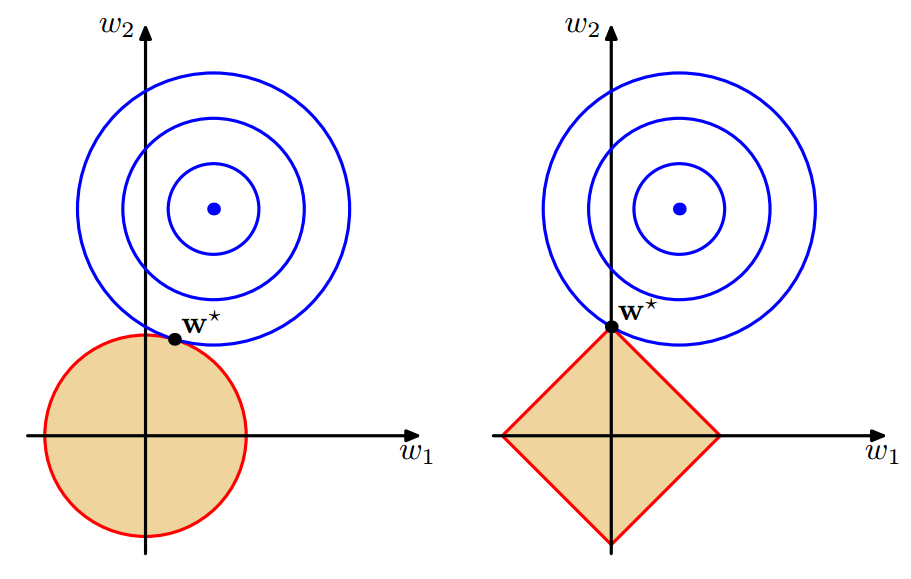
\includegraphics[scale=0.5]{/home/djn_dl/Desktop/GitHub/Commentarii/PRML/1524666731026} 

Think about this figure in a Langrange-multipliers way.

\paragraph{Multiple outputs}

Of course we can decouple into multiple, 1``independent regression
problems, however there is an approach using the same set of basis
functions so that y

\[
y(x,w)=W^{T}\phi(x)
\]

and

\[
p(\mathrm{t}|x,W,\beta)=\mathcal{N}(\mathrm{t}|W^{T}\phi(x),\beta^{-1}I)
\]

which yields

\[
W_{ML}=\Phi^{\dagger}T
\]

For the case of arbitrary covariance matrices, see MAL of multi-variate
Gaussian distribution.
\end{document}
